\section{Documentos}

\subsection[]{Comandos Básicos}

% =============== %
%     Frame       %
\begin{frame}[fragile]
\frametitle{Notas}

\begin{itemize}
  \item Comandos: \verb|\command|, \verb|\command{}|, \verb|\command[]{}|
  \item Ambientes: \verb|\begin{ambiente}...\end{ambiente}|
  \item Caracteres especiais: \verb|$&%#_{}~^\| devem ser precedidos por \verb|\| ou o comando
  \verb|\verb|
  \item Espaçamento automático
  \item Comentários: usa-se o caractere \verb|%| ou \verb|\begin{comment}...\end{comment}|
  \item Delimitador de contexto: \verb|{ ... }|
  \item Referência a arquivos: \verb|/igual/ao/linux|
\end{itemize}
 
\end{frame}


% =============== %
%     Frame       %
\begin{frame}[fragile]
\frametitle{Exemplo funcional mínimo!}

\begin{block}{\LaTeX~hello world!}
\begin{verbatim}
	\documentclass[12pt,a4paper]{article}
	\begin{document}
		Hello world !
	\end{document}
\end{verbatim}
\end{block}
 
\end{frame}

% =============== %
%     Frame       %
\begin{frame}[fragile]
\frametitle{Detalhes do Exemplo}

\begin{block}{Opções}
\begin{verbatim} 
	10pt, 12pt, oneside, twoside, a4paper, 
	letterpaper, titlepage, twocolumn
\end{verbatim}
\end{block}
 \begin{block}{Documentos comuns}
\begin{verbatim} 
	article, book, report, slides, letter
\end{verbatim}
\end{block}
\end{frame}

% =============== %
%     Frame       %
\begin{frame}
\frametitle{O Processo de Compilação}


\begin{figure}
\centering
 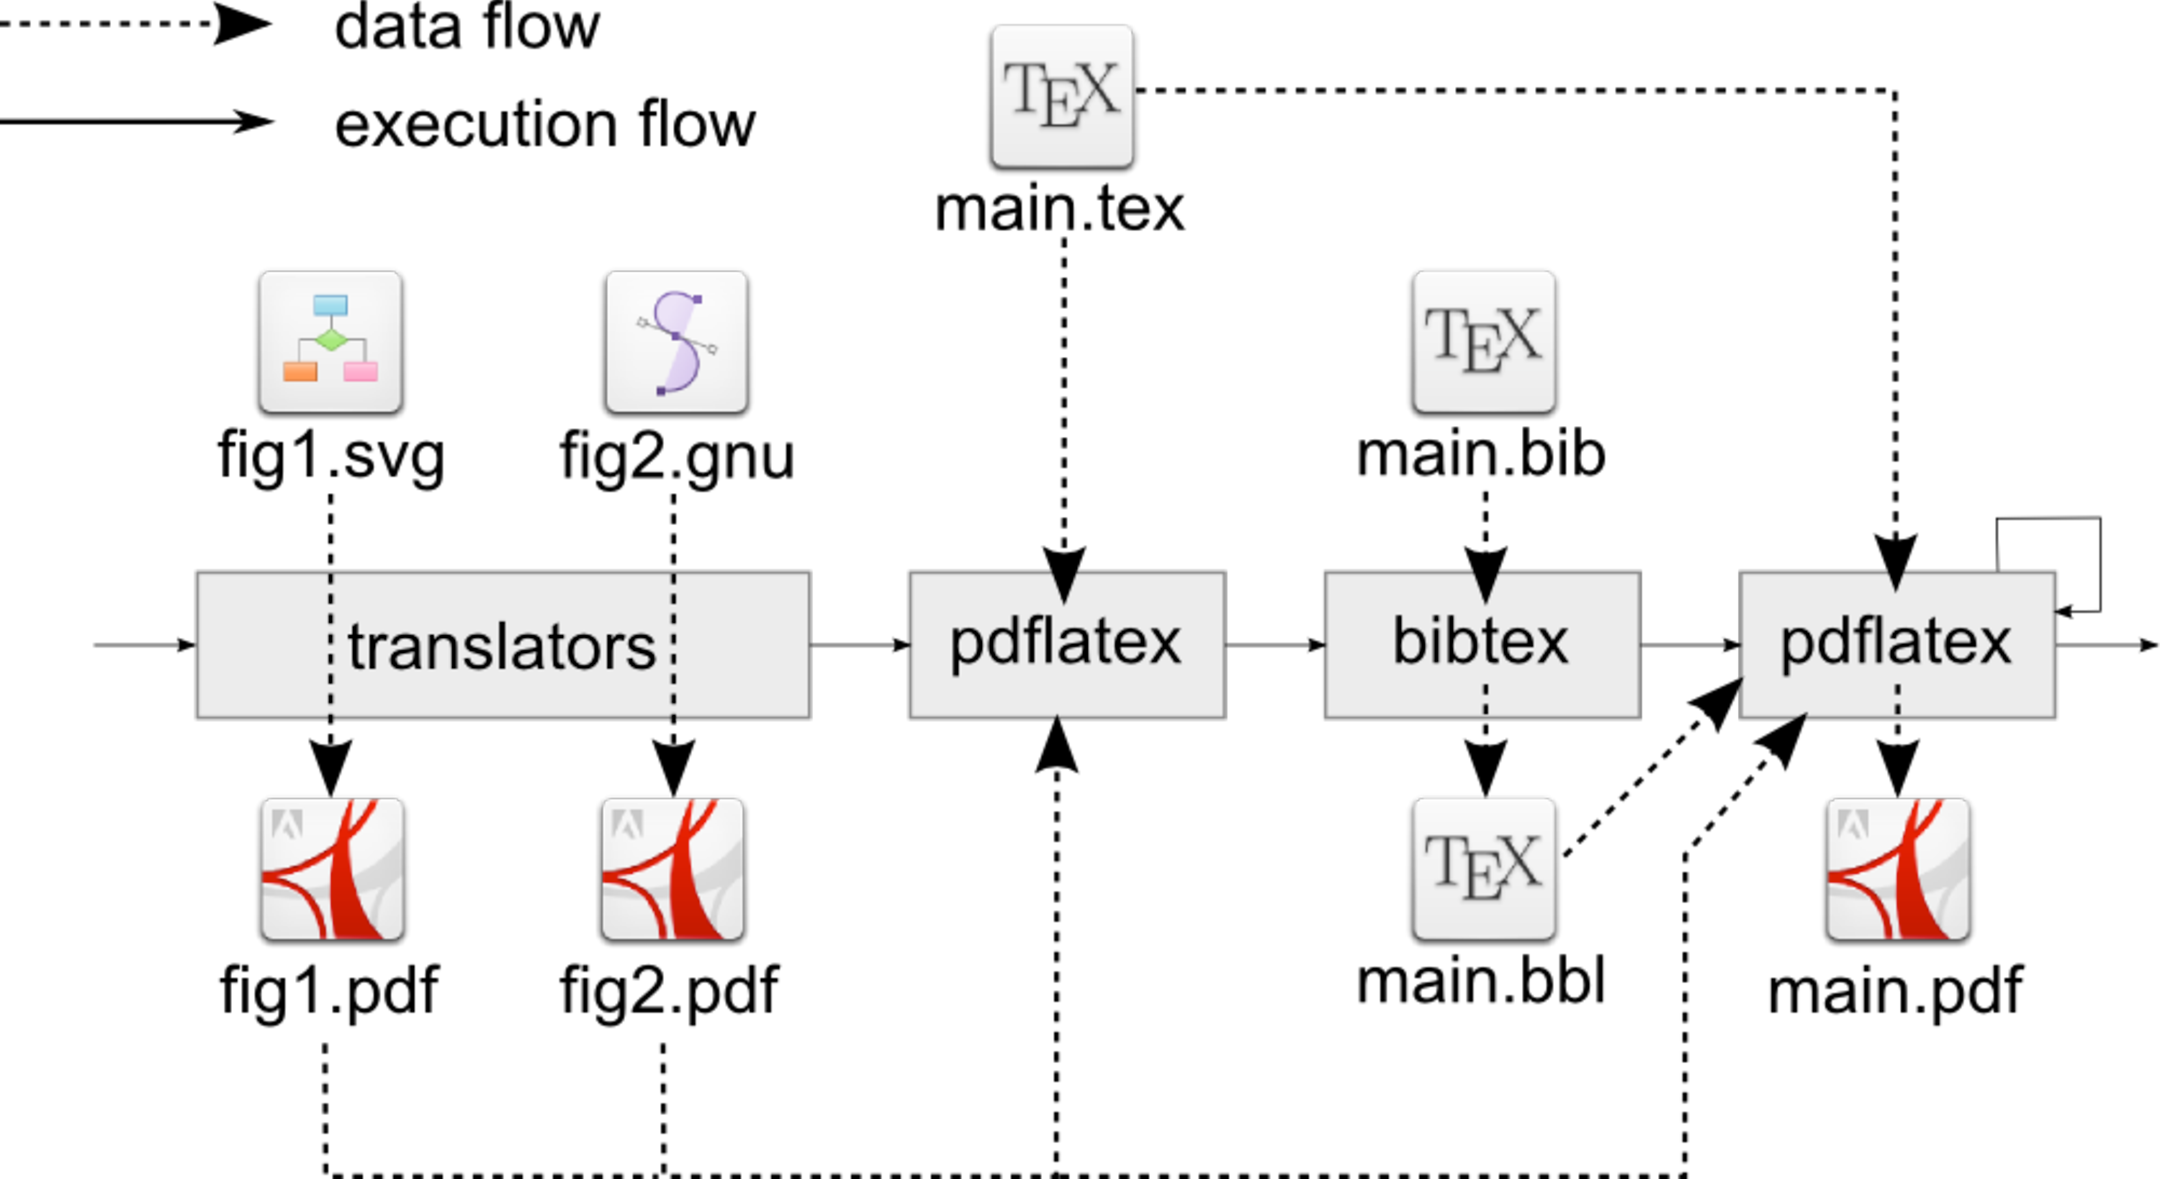
\includegraphics[scale=.25]{../img/process.pdf}
\end{figure}
 
\end{frame}

% =============== %
%     Frame       %
\begin{frame}[fragile]
\frametitle{}

% You can create overlays
\begin{itemize}
  \item O programa \texttt{latex} gera o arquivo \texttt{.dvi}: \texttt{latex arquivo.tex}
  \item A inclusão de referências bibliográficas feita através do programa \texttt{bibtex}:
  \texttt{bibtex arquivo}
  \item O \textit{PostScript} final pode ser gerado pelo \texttt{dvips}: \texttt{dvips arquivo.dvi
  -o arquivo.ps}
  \item O \textit{PostScript} pode ser visualizado e impressão pelo \texttt{gsview32.exe} (Windows)
  ou \texttt{gv} (Linux/Unix).
  \item Uma outra alternativa é utilizar o comando \texttt{pdflatex}
\end{itemize}
 
\end{frame}

% =============== %
%     Frame       %
\begin{frame}
\frametitle{Arquivos Comuns (1/2)}

\begin{itemize}
  \item \texttt{.tex}: Arquivos fontes
  \item \texttt{.log}: Relatório da compilação
  \item \texttt{.dvi}: Resultado da compilação dos arquivos fonte via \textit{latex}
  \item \texttt{.aux}: Arquivos auxiliar utilizado na geração documento final (\textit{.dvi} ou
  	\textit{.pdf})
  \item \texttt{.cls}: Arquivos de classe
  \item \texttt{.sty}: Pacotes
\end{itemize}
 
\end{frame}

% =============== %
%     Frame       % 
\begin{frame}
\frametitle{Arquivos Comuns (2/2)}

% You can create overlays
\begin{itemize}
  \item \texttt{.toc}: Itens para o sumário
  \item \texttt{.lof}: Itens para a lista de figuras
  \item \texttt{.lot}: Itens para a lista de tabelas
  \item \texttt{.bbl}: Itens para a lista de bibliografias
  \item \texttt{.blg}: Arquivos auxiliar utilizado na geração de bibliografias
\end{itemize}
 
\end{frame}


\subsection[]{Elaboração de documentos}\label{sec:elaboracao}
% =============== %
%     Frame       %
\begin{frame}[fragile]
\frametitle{Partes do Documento}

% You can create overlays
\begin{itemize}
  \item Tipos de divisões: \verb|\section{}|, \verb|\subsection{}|, \verb|\subsubsection{}|
\verb|\paragraph{}|, \verb|\subparagraph{}|
  \item Classe book: \verb|\part{}|, \verb|\chapter{}|
  \item Apêndices: \verb|\appendix|
\end{itemize}
 
\end{frame}

% =============== %
%     Frame       %
\begin{frame}[fragile]
\frametitle{Acentuando em Português}

% You can create overlays
\begin{itemize}
  \item Utilizar o pacote babel e fontes especiais: 
  \begin{verbatim}
  	\documentclass[12pt,a4paper]{article} 
  	\usepackage[latin1]{inputenc}
  	\usepackage[T1]{fontenc} 
  	\usepackage[brazil,english]{babel}
  	\begin{document} 
  	\selectlanguage{brazil}
  	...
  	\end{document}
  \end{verbatim}
\end{itemize}
 
\end{frame}

% =============== %
%     Frame       %
\begin{frame}[fragile]
\frametitle{Aplicando Formatações ao Texto}

% You can create overlays
\begin{itemize}
  \item Novo parágrafo: é suficiente deixar uma linha em branco 
  \item Negrito:  \verb|\textbf{text}| $\rightarrow$ \textbf{text}
  \item Itálico:  \verb|\textit{text}| $\rightarrow$ \textit{text}
  \item Texto centralizado, esquerda e direita: Usar ambientes \textit{center}, \textit{flushleft} e
 \textit{flushright}.
 \begin{verbatim}
     \begin{center}
     ... texto ...
     \end{center}
 \end{verbatim}
\end{itemize}
 
\end{frame}

% =============== %
%     Frame       %
\begin{frame}[fragile]
\frametitle{Gerando Listas}

% You can create overlays
\begin{itemize}
  \item Listas numeradas:
\end{itemize}
\begin{columns}
	\column{.5\textwidth}
\begin{verbatim}
	\begin{enumerate}
		\item Banana
		\item Batata
	\end{enumerate}
\end{verbatim}
	\column{.5\textwidth}
	\begin{framed}
	\begin{enumerate}
 		\item Banana
 		\item Batata
 	\end{enumerate}
	\end{framed}
\end{columns}
\end{frame}
	
	
% =============== %
%     Frame       %
\begin{frame}[fragile]
\frametitle{Gerando Listas}

% You can create overlays
\begin{itemize}
  \item Listas de itens:
\end{itemize}
\begin{columns}
	\column{.5\textwidth}
\begin{verbatim}
	\begin{itemize}
		\item Banana
		\item Batata
	\end{itemize}
\end{verbatim}
	\column{.5\textwidth}
	\begin{framed}
	\begin{itemize}
 		\item Banana
 		\item Batata
 	\end{itemize}
	\end{framed}
\end{columns}
\end{frame}


% =============== %
%     Frame       %
\begin{frame}[fragile]
\frametitle{Gerando Listas}

% You can create overlays
\begin{itemize}
  \item Listas de descrição:
\end{itemize}
\begin{columns}
	\column{.5\textwidth}
\begin{verbatim}
	\begin{description}
		\item[Fruta:] Banana
		\item[Ferramenta:] Martelo
	\end{description}
\end{verbatim}
	\column{.5\textwidth}
	\begin{framed}
	\begin{description}
		\item[Fruta:] Banana
		\item[Ferramenta:] Martelo
	\end{description}
	\end{framed}
\end{columns}
\end{frame}
	
% =============== %
%     Frame       %
\begin{frame}[fragile]
\frametitle{Edição Matemática Básica}

% You can create overlays
\begin{itemize}
  \item Modo texto $V.S$ modo matemático
  \item Separadores \verb|$ ... $| e \verb|$$ ... $$|: 
\end{itemize}
\begin{columns}
	\column{.5\textwidth}
\begin{verbatim}
	  Tem-se que $x=0$.
\end{verbatim}
	\column{.5\textwidth}
	\begin{framed}
	Tem-se que $x=0$.
	\end{framed}
\end{columns}
\begin{columns}
	\column{.5\textwidth}
\begin{verbatim}
	  Tem-se que: $$x=0$$.
\end{verbatim}
	\column{.5\textwidth}
	\begin{framed}
	Tem-se que: $$x=0$$.
	\end{framed}
\end{columns}

\end{frame}


% =============== %
%     Frame       %
\begin{frame}[fragile]
\frametitle{Edição Matemática Básica}

% You can create overlays
\begin{itemize}
  \item Sobrescrito e Subescrito:
      
\begin{columns}
\small
	\column{.6\textwidth}
\verb|$X^{sup}=Y_{inf}=Z^{sup}_{inf}$|
	\column{.4\textwidth}
	\begin{framed}
	$X^{sup}=Y_{inf}=Z^{sup}_{inf}$
	\end{framed}
\end{columns}

\item Espaços em modo matemático:
\begin{columns} \small
	\column{.6\textwidth}
	\verb|$a b,a\;b,a\;\;\;b$| 
	\column{.4\textwidth}
	\begin{framed}
	$a b,a\;b,a\;\;\;b$ 
	\end{framed}
\end{columns}

\item Negrito:
\begin{columns}\small
	\column{.6\textwidth}
\verb|$\mathbf{x} = [x_1 \;\; x_2]^T$|
	\column{.4\textwidth}
	\begin{framed}
	$\mathbf{x} = [x_1 \;\; x_2]^T$
	\end{framed}
\end{columns}
\end{itemize}
\end{frame}


% =============== %
%     Frame       %
\begin{frame}[fragile]
\frametitle{Edição Matemática Básica}

% You can create overlays
\begin{itemize}
  \item Vetores:
      
\begin{columns}
\small
	\column{.6\textwidth}
\begin{verbatim}
$$\vec{a},\hat{a},\bar{a},
\tilde{a},\dot{a},\ddot{a}$$
\end{verbatim}
	\column{.4\textwidth}
	\begin{framed}
	$$\vec{a},\hat{a},\bar{a},
	\tilde{a},\dot{a},\ddot{a}$$
	\end{framed}
\end{columns}

\item Somatórios e Integrais:
\begin{columns} \small
	\column{.6\textwidth}
	\begin{verbatim}
	$$\sum_{i=1}^{n}f(x_i)\Delta x 
	\approx \int_a^bf(x)dx$$
	\end{verbatim}
	\column{.4\textwidth}
	\begin{framed}
	 $$\sum_{i=1}^{n}f(x_i)\Delta x
	  \approx \int_a^bf(x)dx$$
	\end{framed}
\end{columns}

\end{itemize}
\end{frame}

% =============== %
%     Frame       %
\begin{frame}[fragile]
\frametitle{Edição Matemática Básica}

% You can create overlays
\begin{itemize}
	\item Frações:
	\begin{columns}
	\small
	\column{.6\textwidth}
	 \verb|$$(y+2)\frac{x+1}{x-1}$$|
	 \column{.4\textwidth}
	\begin{framed}
	$$(y+2)\frac{x+1}{x-1}$$
	\end{framed}	 
	 \end{columns}
	
	\item Limites e derivadas parciais: {\small
	\begin{verbatim}
$$\frac{\partial f(x,y)}{\partial x} =
\lim_{\Delta x \to 0}\frac{f(x+\Delta x,y)-
f(x,y)}{\Delta x}$$
	\end{verbatim}
	\begin{framed}
	$$\frac{\partial f(x,y)}{\partial x} =
\lim_{\Delta x \to 0}\frac{f(x+\Delta x,y)-
f(x,y)}{\Delta x}$$
	\end{framed}	
	}

\end{itemize}
 
\end{frame}
% =============== %
%     Frame       %
\begin{frame}[fragile]
\frametitle{Edição Matemática Básica}

% You can create overlays
\begin{itemize}
  \item Parênteses, chaves e colchetes:
  	\begin{columns}
	\small
	\column{.5\textwidth}
	\begin{verbatim}	
$$ \left[
   \left\{
     \left(
       {1 \over x}
     \right)^2 - 3
   \right\} + x^2
 \right]^3
 $$
	\end{verbatim}
	\column{.5\textwidth}
	\begin{framed}
	$$ \left[
   \left\{
     \left(
       {1 \over x}
     \right)^2 - 3
   \right\} + x^2
 \right]^3
 $$
	\end{framed}
 \end{columns}
\end{itemize}
 
\end{frame}

% =============== %
%     Frame       %
\begin{frame}[fragile]
\frametitle{Edição Matemática Básica}

% You can create overlays
\begin{itemize}
  \item Matrizes:  \textit{\color{oliveGreen}//Definição}
\begin{verbatim}
$$\mathbf{I} =
\left[
  \begin{array}{cccc}
  1      & 0      & \ldots & 0      \\
  0      & 1      & \ldots & 0      \\
  \vdots & \vdots & \ddots & \vdots \\
  0      & 0      & \ldots & 1
  \end{array}
\right]$$
\end{verbatim}
\end{itemize}
 
\end{frame}

% =============== %
%     Frame       %
\begin{frame}[fragile]
\frametitle{Edição Matemática Básica}

% You can create overlays
\begin{itemize}
  \item Matrizes:  \textit{\color{oliveGreen}//Resultado}
$$\mathbf{I} =
\left[
  \begin{array}{cccc}
  1      & 0      & \ldots & 0      \\
  0      & 1      & \ldots & 0      \\
  \vdots & \vdots & \ddots & \vdots \\
  0      & 0      & \ldots & 1
  \end{array}
\right]$$
\end{itemize}
 
\end{frame}

% =============== %
%     Frame       %
\begin{frame}[fragile]
\frametitle{Edição de Tabelas}


\begin{itemize}
  \item Ambiente \texttt{tabular}: {\color{oliveGreen} \textit{//Definição}}
 {\small
  \begin{verbatim}
\begin{tabular}{||l|c|c|r||} 
\hline
 Item & Preço & Quantidade & Total \\ 
\hline \hline
Banana & 0,55 & 5 & 2,75  \\
\hline
Batata & 0,35 & 3 & 1,05  \\
\hline \hline
       &      & Total & 3,80  \\
\hline
\end{tabular}  
  \end{verbatim}
 }
\end{itemize}
\end{frame}
% =============== %
%     Frame       %
\begin{frame}[fragile]
\frametitle{Edição de Tabelas}

\begin{itemize}
  \item Ambiente \texttt{tabular}: {\color{oliveGreen} \textit{//Resultado}}
  \newline
  \newline
\begin{tabular}{|l|c|c|r|} 
\hline
 Item & Preço & Quantidade & Total \\ 
\hline
Banana & 0,55 & 5 & 2,75  \\
\hline
Batata & 0,35 & 3 & 1,05  \\
\hline 
& & Total & 3,80 \\
\hline
\end{tabular}  
\end{itemize}
\end{frame}


% =============== %
%     Frame       %
\begin{frame}[fragile]
\frametitle{Incluindo Figuras}

\begin{itemize}
  \item Declarar o pacote \texttt{graphicx}: \verb|\usepackage{graphicx}|
  \item Inserir o comando \verb|\includegraphics[options]{path}|:
  \item Exemplo:
  {\small
  \begin{verbatim}
\includegraphics[scale=.3] {figs/leslie.ps}
  \end{verbatim}
  }
  \item Outras opções disponíveis: \textit{scale},\textit{width}, \textit{height} e \textit{angle}.
\end{itemize}
 
\end{frame}

% =============== %
%     Frame       %
\begin{frame}[fragile]
\frametitle{Mudando o tipo de fonte}

\begin{table}
\centering
\begin{tabular}{ll}
\toprule
\textbf{Comando} & \textbf{Família de fonte} \\
\midrule
\verb|\textit{Itálico}| & \textit{Itálico} \\
\verb|\textsc{Small Caps}| & \textsc{Small Caps} \\
\verb|\textbf{Negrito}| & \textbf{Negrito} \\
\verb|\texttt{Typewriter}| & \texttt{Typewriter} \\
\verb|\textsf{Sans Serif} | & \textsf{Sans Serif}\\
\verb|\textrm{Romano}| & \textrm{Romano} \\
\verb|\textsl{Inclinado}| & \textsl{Inclinado} \\
\bottomrule
\end{tabular}
\end{table}
 
\end{frame}

% =============== %
%     Frame       %
\begin{frame}[fragile]
\frametitle{Mudando o tamanho da fonte}

\begin{table}
\centering
\begin{tabular}{ll}
\toprule
\textbf{Comando} & \textbf{Tamanho resultante	} \\
\midrule
\verb|{\tiny LES}| &  {\tiny LES}\\
\verb|{\scriptsize LES}| & {\scriptsize LES} \\
\verb|{\footnotesize LES}| & {\footnotesize LES} \\
\verb|{\small LES}| & {\small LES} \\
\verb|{\normal LES}| & {\normal LES} \\
\verb|{\large LES}| & {\large LES} \\
\verb|{\Large LES}| & {\Large LES} \\
\verb|{\LARGE LES}| & {\LARGE LES} \\
\verb|{\huge LES}| & {\huge LES} \\
\verb|{\Huge LES}| & {\Huge LES} \\
\bottomrule
\end{tabular}
\end{table}
 
\end{frame}

% =============== %
%     Frame       %
\begin{frame}[fragile]
\frametitle{Estilo de Páginas}


\begin{itemize}
  \item O comando \verb|\pagestyle{}| define a aparência das páginas:
  \begin{itemize}
    \item \verb|\pagestyle{plain}|: Numeração no rodapé e sem cabeçalho.
    \item \verb|\pagestyle{headings}|: Numeração no rodapé e cabeçalho.
    \item \verb|\pagestyle{empty}|: Sem numeração ou cabeçalho.
    \item \verb|\pagestyle{myheadings}|: Permite que o usuário especifique através dos comandos
    \verb|\markboth{cab_esq}{cab_dir}| e \verb|\markright{cab_dir}|.
    \item Use \verb|\thispagestyle{estilo}| para mudar somente uma determinada página.
  \end{itemize}
\end{itemize}
 
\end{frame}

% =============== %
%     Frame       %
\begin{frame}[fragile]
\frametitle{Uma capa mínima e sumário}

\begin{itemize}
  \item Incluir \texttt{titlepage} nas opções de classe
  \item Definir o \textit{título} do trabalho, \textit{autor} e \textit{data}: 
\verb|\title{Curso de \LaTeX}|
\verb|\author{Alcemir Santos}|
\verb|\date{}|, \verb|\date{\today}| ou \verb|\date{Outubro/2008}|
  \item Colocar o comando \verb|\maketitle| depois do início do documento.
  \item Acrescentar a seguir o comando \verb|\tableofcontents|
\end{itemize}
 
\end{frame}
% =============== %
%     Frame       %
\begin{frame}[fragile]
\frametitle{Espaçamentos}

\begin{itemize}
	\item Horizontais:
	\item[] Efeito do comando \verb|\hspace{.83cm}|\hspace{.83cm} na linha
	\item[] Efeito do comando \verb|\hfill|\hfill na linha
	\item[] Efeito do comando \verb|\hrulefill|\hrulefill na linha
	\item[] Efeito do comando \verb|\dotfill|\dotfill na linha
	\item Verticais:
	\item[] Espaçamento fixo: \verb|\vspace{0.3cm}|\vspace{0.3cm}
	\item[] Preenchimento vertical: \verb|\vfill|\vfill
	\item \verb|\hspace*{}| e \verb|\vspace*{}| $\rightarrow$ evitam problemas com linha nova e página
nova
\end{itemize}
 
\end{frame}

% =============== %
%     Frame       %
\begin{frame}[fragile]
\frametitle{Mais formatação}

\begin{itemize}
  \item Se a hifenação falhar, colocar no preâmbulo: \verb|\hyphenation{hi-fen ma-nu-al}|
  \item O comando \verb|\pagebreak| inicia um nova página
  \item Notas de rodapé\footnote{como esta aqui em baixo.} podem ser feitas com
  \verb|\footnote{texto}|
\end{itemize}
 
\end{frame}

% =============== %
%     Frame       %
\begin{frame}[fragile]
\frametitle{Objetos Flutuantes}
\begin{columns}
	\small
	\column{.5\textwidth}
\begin{block}{Tabelas}
\begin{verbatim}
	\begin{table}[h|t|b|p]
\begin{tabular}
  ...
\end{tabular}
\end{table}
\end{verbatim}
\end{block}

	 \column{.5\textwidth}
\begin{block}{Figuras}
\begin{verbatim}
\begin{figure}[h|t|b|p] 
... 
\includegraphics{}
... 
\end{figure}
\end{verbatim}
\end{block}
\end{columns}

\begin{itemize}
  \item  \verb|\clearpage|
  \item[] Finaliza a página e força o aparecimento dos objetos flutuantes
  restantes
\end{itemize}
 
\end{frame}


% =============== %
%     Frame       %
\begin{frame}[fragile]
\frametitle{Multiplas Figuras}

Permite que várias figuras sejam agrupadas em uma só área.
    \begin{itemize}
    	\item \verb|\usepackage{subfigure}|
    \end{itemize}
    
\begin{verbatim}
\begin{figure}
\mbox{
    \subfigure[Caption (a)]{  
        \includegraphics[scale=.3]{fig-a.ps}  }
    \subfigure[caption (b)]{ 
        \includegraphics[scale=.3]{fig-b.ps}  }
}
\caption{Caption geral}
\end{figure}
\end{verbatim}

 
\end{frame}
% =============== %
%     Frame       %
\begin{frame}[fragile]
\frametitle{Algoritmos}

Permite a inclusão de arquivos com código\hyp{}fonte no documento, com formatação
  dependente da linguagem.
  \begin{verbatim}
  	\usepackage{listings}, \lstloadlanguages{C},
  	\lstset{language=C}, \lstinputlisting{filename}
  \end{verbatim}

\begin{framed}
\small
\begin{lstlisting}
#include <stdio.h>
/* Comment block */
int main(){
    // Line comment.
    printf("LaTeX is great for programmers!"));
    return 0;
}
\end{lstlisting} 
\end{framed}
\end{frame}

% =============== %
%     Frame       %
\begin{frame}[fragile]
\frametitle{Referências Cruzadas}

\begin{itemize}
  \item \verb|\label{ELEM-ID}|: Relaciona o elemento corrente do documento com a chave
  \texttt{ELEM-ID}.
  \item  Pode ser tabelas, figuras, seções, subseções, item de lista, \textit{etc}.
  \item \verb|\ref{ELEM-ID}|: Referencia o elemento relacionado com a chave \texttt{ELEM-ID}
  \item \verb|\pageref{ELEM-ID}|: Referencia a página onde está o elemento relacionado com
  a chave \texttt{ELEM-ID}
  \item As chaves devem ser únicas e são sensíveis à caixa
  \item Deve-se compilar duas vezes
\end{itemize}
 
\end{frame}


% =============== %
%     Frame       %
\begin{frame}[fragile]
\frametitle{Referências Cruzadas: tabelas}
{\scriptsize
\begin{columns}
\column{.5\textwidth}
\begin{verbatim}
\begin{table}
\centering
\begin{tabular}{|c|c|}\hline
Quant & R\$  \\ \hline
10    & 2.3  \\ \hline
\end{tabular}
\caption{Valores}
\label{tab:valores}
\end{table}

A Tabela~\ref{tab:valores} 
mostra \ldots
\end{verbatim}

\column{.5\textwidth}
\begin{table}
\centering
\begin{tabular}{|c|c|}\hline
Quant & R\$  \\ \hline
10    & 2.3  \\ \hline
\end{tabular}
\caption{Valores}
\label{tab:valores}
\end{table}

A Tabela~\ref{tab:valores} mostra \ldots
\end{columns}
 }
\end{frame}


% =============== %
%     Frame       %
\begin{frame}[fragile]
\frametitle{Referências Cruzadas: figuras}
{\scriptsize
\begin{columns}
\column{.5\textwidth}
\begin{verbatim}
\begin{figure}
  \centering
  
\includegraphics[scale=.3]
  {./img/les}
  \caption{Logo do LES.}
  \label{fig:les}
\end{figure}
A Figura~\ref{fig:les} 
(Pág. \pageref{fig:les})
 mostra \ldots

A Figura~\ref{fig:les} 
mostra \ldots
\end{verbatim}

\column{.5\textwidth}
\begin{figure}
  \centering
  
\includegraphics[scale=.3]{../img/les.pdf}
  \caption{Logo do LES.}
  \label{fig:les}
\end{figure}
A Figura~\ref{fig:les} 
(Pág. \pageref{fig:les})
 mostra \ldots
\end{columns}
}
\end{frame}

% =============== %
%     Frame       %
\begin{frame}[fragile]
\frametitle{Referências Cruzadas: equações}
{\scriptsize
\begin{columns}
\column{.5\textwidth}
\begin{verbatim}
A Equação~\ref{eq:logn} mostra a definição
da  função logaritmo , válida
para $x>0$.

\begin{equation}
\ln(x)=\int_1^x
{1 \over t}dt
\label{eq:logn}
\end{equation}
\end{verbatim}

\column{.5\textwidth}
\begin{framed}
A Equação~\ref{eq:logn} mostra
a definição da função logaritmo,
válida para $x>0$.

\begin{equation}
\ln(x)=\int_1^x
{1 \over t}dt
\label{eq:logn}
\end{equation}
\end{framed}
\end{columns}
 }
\end{frame}

% =============== %
%     Frame       %
\begin{frame}[fragile]
\frametitle{Referências Cruzadas: equações}

Na início da seção adicionei o comando \verb|\label{}| após a definição da seção com
\verb|\section{}| assim:
\begin{verbatim}
\section{Minha seção} \label{sec:minha}
\end{verbatim}

A referência a esta seção deve ser feita assim:

\begin{columns}
\column{.5\textwidth}
\begin{verbatim}

A Seção \ref{sec:minha} 
apresenta \ldots

\end{verbatim}

\column{.5\textwidth}
\begin{framed}
A Seção \ref{sec:elaboracao}
apresenta \ldots
\end{framed}
\end{columns}
\end{frame}


% =============== %
%     Frame       %
\begin{frame}[fragile]
\frametitle{Referências Bibliográficas}

\begin{enumerate}
  \item Criar um arquivo de bibliografias (\textit{.bib})
  \item Utilizar o comando \verb|\cite{chave}| para indicar a referência bibliográfica desejada
  \item Definir o estilo de referência utilizada com \verb|\bibliographystyle{estilo}|
  \item Especificar o arquivo de bibliografias e o ponto de inserção com
  \verb|\bibliography{arquivo}|
  \item Utilizar o \texttt{bibtex}, compilador de referências
\end{enumerate}
 
\end{frame}

% =============== %
%     Frame       %
\begin{frame}[fragile]
\frametitle{Arquivo de Bibliográfias}

\begin{itemize}
  \item Formato:
  \begin{framed}
  \begin{verbatim}
	@tipo_de_citação{chave, 
	 campo_1 = {Valor 1},
	 campo_2 = {Valor 2},
	 ...,
     campo_n = {Valor n},
	}
  \end{verbatim}
  \end{framed}
  \item Tipos mais comuns: \textit{book}, \textit{article}, \textit{inproceedings},
  \textit{inbook}, \textit{masterthesis},
  \textit{phdthesis}, \textit{techreport}.
\end{itemize}
 
\end{frame}

% =============== %
%     Frame       %
\begin{frame}[fragile]
\frametitle{Citando Referências}


\begin{itemize}
  \item \verb|\cite{chave}|: coloca a chamada da referência e inclui na lista final
  \item \verb|\nocite{chave}|: não coloca a chamada mas inclui na lista
  \item \verb|\nocite{*}|: lista todas as referências bibliográficas sem chamada no texto
  \item[] 
  \item Leitura adicional: pacote \texttt{natbib}.
\end{itemize}
 
\end{frame}

% =============== %
%     Frame       %
\begin{frame}
\frametitle{Exercícios}


\begin{enumerate}
  \item Elaborar um documento com as estruturas vistas até aqui.
  \item Criar artigo com template\footnote{Disponível aqui: \url{http://bit.ly/1BQBTq9}} da
  Sociedade Brasileira de Computação.
\end{enumerate}
 
\end{frame}

